\documentclass[conference]{IEEEtran}
\IEEEoverridecommandlockouts
\usepackage{cite}
\usepackage[T1]{fontenc}
\usepackage{newtxtext,newtxmath}
\usepackage{amsmath}
\usepackage{graphicx}
\usepackage{booktabs}
\usepackage{xcolor}
\usepackage{url}
\usepackage[hidelinks]{hyperref}
% generated by experiments/report.py -- do not edit
\newcommand{\NRows}{259,181}
\newcommand{\NQueries}{43,443}
\newcommand{\NCrops}{49}
\newcommand{\NStates}{36}
\newcommand{\NDistricts}{748}
\newcommand{\YearA}{1997}
\newcommand{\YearB}{2022}
\newcommand{\KaggleRF}{99.5}
\newcommand{\KaggleNB}{99.5}
\newcommand{\StatesN}{32}
\newcommand{\StatesBelowIID}{4}
\newcommand{\StatesBelowGRP}{4}
\newcommand{\OursNDCGR}{0.936}
\newcommand{\OursHitR}{59.7}
\newcommand{\OursHitThreeR}{89.9}
\newcommand{\BaseNDCGR}{0.915}
\newcommand{\BaseHitR}{57.5}
\newcommand{\BaseHitThreeR}{88.6}
\newcommand{\BaseNameR}{Random Forest}
\newcommand{\GainHitR}{2.2}
\newcommand{\GainNDCGR}{0.021}
\newcommand{\PersNDCGR}{0.914}
\newcommand{\PersHitR}{55.3}
\newcommand{\PHitR}{=1.0\times10^{-23}}
\newcommand{\NPairedR}{43,443}
\newcommand{\CovIIDR}{90.3}
\newcommand{\CovGRPR}{90.1}
\newcommand{\SizeIIDR}{2.65}
\newcommand{\SizeGRPR}{2.64}
\newcommand{\APSCovGRPR}{91.3}
\newcommand{\APSSizeGRPR}{3.81}
\newcommand{\OursNDCGLSO}{0.922}
\newcommand{\OursHitLSO}{55.6}
\newcommand{\OursHitThreeLSO}{88.0}
\newcommand{\BaseNDCGLSO}{0.833}
\newcommand{\BaseHitLSO}{38.5}
\newcommand{\BaseHitThreeLSO}{74.1}
\newcommand{\BaseNameLSO}{MLP}
\newcommand{\GainHitLSO}{17.0}
\newcommand{\GainNDCGLSO}{0.089}
\newcommand{\PersNDCGLSO}{0.909}
\newcommand{\PersHitLSO}{54.5}
\newcommand{\PHitLSO}{<10^{-300}}
\newcommand{\NPairedLSO}{43,443}
\newcommand{\CovIIDLSO}{90.1}
\newcommand{\CovGRPLSO}{89.6}
\newcommand{\SizeIIDLSO}{2.87}
\newcommand{\SizeGRPLSO}{2.82}
\newcommand{\APSCovGRPLSO}{90.0}
\newcommand{\APSSizeGRPLSO}{3.98}
\newcommand{\OursNDCGLYO}{0.930}
\newcommand{\OursHitLYO}{57.8}
\newcommand{\OursHitThreeLYO}{89.0}
\newcommand{\BaseNDCGLYO}{0.897}
\newcommand{\BaseHitLYO}{52.1}
\newcommand{\BaseHitThreeLYO}{84.2}
\newcommand{\BaseNameLYO}{XGBoost}
\newcommand{\GainHitLYO}{5.8}
\newcommand{\GainNDCGLYO}{0.033}
\newcommand{\PersNDCGLYO}{0.914}
\newcommand{\PersHitLYO}{55.2}
\newcommand{\PHitLYO}{=5.3\times10^{-136}}
\newcommand{\NPairedLYO}{43,443}
\newcommand{\CovIIDLYO}{89.4}
\newcommand{\CovGRPLYO}{89.7}
\newcommand{\SizeIIDLYO}{2.67}
\newcommand{\SizeGRPLYO}{2.71}
\newcommand{\APSCovGRPLYO}{91.2}
\newcommand{\APSSizeGRPLYO}{4.01}
\newcommand{\MedianCand}{5}
\newcommand{\MaxCand}{27}
\newcommand{\MeanCand}{6.0}
\newcommand{\WorstFirstYear}{1997}
\newcommand{\WorstCand}{9.2}
\newcommand{\ColdShareR}{39.7}
\newcommand{\OursHitColdR}{53.1}
\newcommand{\OursHitWarmR}{64.0}
\newcommand{\BaseHitColdR}{48.5}
\newcommand{\PersPColdR}{=4.9\times10^{-109}}
\newcommand{\PersPWarmR}{=8.5\times10^{-11}}
\newcommand{\PersPR}{=3.7\times10^{-91}}
\newcommand{\PersHitColdR}{44.5}
\newcommand{\PersHitWarmR}{62.4}
\newcommand{\ColdShareLSO}{39.7}
\newcommand{\OursHitColdLSO}{47.2}
\newcommand{\OursHitWarmLSO}{61.0}
\newcommand{\BaseHitColdLSO}{32.2}
\newcommand{\PersPColdLSO}{=1.1\times10^{-33}}
\newcommand{\PersPWarmLSO}{=4.0\times10^{-7}}
\newcommand{\PersPLSO}{=3.2\times10^{-6}}
\newcommand{\PersHitColdLSO}{42.6}
\newcommand{\PersHitWarmLSO}{62.4}
\newcommand{\ColdShareLYO}{39.7}
\newcommand{\OursHitColdLYO}{50.3}
\newcommand{\OursHitWarmLYO}{62.7}
\newcommand{\BaseHitColdLYO}{42.0}
\newcommand{\PersPColdLYO}{=8.4\times10^{-57}}
\newcommand{\PersPWarmLYO}{=1.5\times10^{-1}}
\newcommand{\PersPLYO}{=1.9\times10^{-33}}
\newcommand{\PersHitColdLYO}{44.2}
\newcommand{\PersHitWarmLYO}{62.4}
\newcommand{\RFCovIIDMean}{75.4}
\newcommand{\RFCovIIDMin}{67.2}
\newcommand{\RFCovIIDMax}{84.8}
\newcommand{\RFCovGRPMean}{89.5}
\newcommand{\RFCovGRPMin}{85.3}
\newcommand{\RFCovGRPMax}{92.4}
\newcommand{\RFSizeGRPLSO}{5.00}
\newcommand{\XGBSizeGRPLSO}{4.67}
\newcommand{\PointHitLSO}{56.2}
\newcommand{\PointNDCGLSO}{0.923}
\newcommand{\PointPLSO}{=4.4\times10^{-5}}
\newcommand{\WorstState}{Telangana}
\newcommand{\WorstIID}{74.9}
\newcommand{\WorstGRP}{73.8}
\newcommand{\MedianStateCovIID}{92.4}
\newcommand{\RFHitR}{57.5}
\newcommand{\MLPHitR}{53.7}
\newcommand{\NBHitR}{33.1}
\newcommand{\XGBHitR}{57.5}
\newcommand{\RFHitLSO}{36.3}
\newcommand{\MLPHitLSO}{38.5}
\newcommand{\NBHitLSO}{26.6}
\newcommand{\XGBHitLSO}{38.2}
\newcommand{\RFHitLYO}{52.0}
\newcommand{\MLPHitLYO}{50.5}
\newcommand{\NBHitLYO}{31.6}
\newcommand{\XGBHitLYO}{52.1}
\newcommand{\SoilOwnPct}{99.8}
\newcommand{\SoilMedPct}{0.2}
\newcommand{\PriorHitR}{29.0}
\newcommand{\PriorHitLSO}{20.8}
\newcommand{\PriorHitLYO}{27.7}
\newcommand{\ClfDropMax}{21.2}
\newcommand{\OursDrop}{4.1}
\newcommand{\NHOursHitR}{54.7}
\newcommand{\NHOursNDCGR}{0.921}
\newcommand{\NHBaseHitR}{53.2}
\newcommand{\NHBaseNDCGR}{0.895}
\newcommand{\NHBaseNameR}{XGBoost}
\newcommand{\NHCovIIDR}{90.1}
\newcommand{\NHOursHitLSO}{27.8}
\newcommand{\NHOursNDCGLSO}{0.788}
\newcommand{\NHBaseHitLSO}{25.6}
\newcommand{\NHBaseNDCGLSO}{0.774}
\newcommand{\NHBaseNameLSO}{MLP}
\newcommand{\NHCovIIDLSO}{77.9}
\newcommand{\NHOursHitLYO}{50.5}
\newcommand{\NHOursNDCGLYO}{0.903}
\newcommand{\NHBaseHitLYO}{46.8}
\newcommand{\NHBaseNDCGLYO}{0.877}
\newcommand{\NHBaseNameLYO}{Random Forest}
\newcommand{\NHCovIIDLYO}{87.7}
\newcommand{\NSRFHitR}{55.9}
\newcommand{\NSXGBHitR}{56.5}
\newcommand{\NSOursHitR}{59.4}
\newcommand{\NSRFHitLSO}{38.8}
\newcommand{\NSXGBHitLSO}{40.8}
\newcommand{\NSOursHitLSO}{55.7}
\newcommand{\NSRFHitLYO}{50.5}
\newcommand{\NSXGBHitLYO}{51.0}
\newcommand{\NSOursHitLYO}{57.2}
\newcommand{\NHRFHitR}{53.1}
\newcommand{\NHRFHitLSO}{25.2}
\newcommand{\NHPriorHitLSO}{20.8}
\newcommand{\CCLACCovR}{90.0}
\newcommand{\CCLACSizeR}{2.62}
\newcommand{\CCAPSCovR}{91.5}
\newcommand{\CCAPSSizeR}{3.82}
\newcommand{\CCHitR}{60.1}
\newcommand{\CCMNCovR}{90.1}
\newcommand{\CCMNSizeR}{2.88}
\newcommand{\CCMRCovR}{90.1}
\newcommand{\CCMRSizeR}{2.66}
\newcommand{\CCLACCovLSO}{89.8}
\newcommand{\CCLACSizeLSO}{2.85}
\newcommand{\CCAPSCovLSO}{90.8}
\newcommand{\CCAPSSizeLSO}{4.21}
\newcommand{\CCHitLSO}{56.1}
\newcommand{\CCMNCovLSO}{90.0}
\newcommand{\CCMNSizeLSO}{3.15}
\newcommand{\CCMRCovLSO}{90.2}
\newcommand{\CCMRSizeLSO}{2.96}
\newcommand{\CCLACCovLYO}{90.1}
\newcommand{\CCLACSizeLYO}{2.70}
\newcommand{\CCAPSCovLYO}{91.1}
\newcommand{\CCAPSSizeLYO}{3.92}
\newcommand{\CCHitLYO}{58.5}
\newcommand{\CCMNCovLYO}{90.1}
\newcommand{\CCMNSizeLYO}{2.98}
\newcommand{\CCMRCovLYO}{89.9}
\newcommand{\CCMRSizeLYO}{2.73}
\newcommand{\CCStatesBelow}{3}
\newcommand{\CCWorstCov}{74.8}
\newcommand{\CCWorstState}{Telangana}
\newcommand{\CCTelanganaCov}{74.8}
\newcommand{\MNStatesBelow}{4}
\newcommand{\MNWorstCov}{78.6}
\newcommand{\MNWorstState}{Haryana}
\newcommand{\MNTelanganaCov}{84.4}
\newcommand{\MRStatesBelow}{3}
\newcommand{\MRWorstCov}{77.3}
\newcommand{\MRWorstState}{Nagaland}
\newcommand{\MRTelanganaCov}{88.6}
\newcommand{\MNAtCCWorst}{84.4}


\begin{document}

\title{Beyond 99\%: Yield-Grounded Crop Ranking with Conformal Prediction Sets, Evaluated on Unseen Indian States and Years}

\author{\IEEEauthorblockN{Rajat Patel, Harshit Jain, Sanyam Jain, Ravi Pratap Singh\textsuperscript{*}, and Imran Khan}
\IEEEauthorblockA{Department of Computer Science and Engineering\\
Harcourt Butler Technical University (HBTU), Kanpur, India\\
Imran Khan is Professor, Dept.\ of CSE, and project supervisor.\\
\textsuperscript{*}Corresponding author: 230104047@hbtu.ac.in}}

\maketitle

\begin{abstract}
Crop-recommendation papers routinely report 97--99.9\% accuracy, almost always on a small,
augmented, location-free table split at random. We ask how such recommenders behave on real data
in states and years they have never seen. From Government of India
district\,$\times$\,season\,$\times$\,year crop statistics joined with NASA POWER climate and
SoilGrids soil, we build a benchmark of \NQueries{} district-season-years (\NCrops{} crops,
\NStates{} states/UTs, \YearA--\YearB). We recast recommendation as \emph{ranking the crops grown in
a district by realised yield}. Four classifier families from the literature, which reach
\KaggleRF\% on the Kaggle table, pick the best-yielding crop in at most \BaseHitR\% of cases under
a random split. On held-out states this falls to \BaseHitLSO\%, below a one-line rule that repeats
last year's yield ranking (\PersHitLSO\%). A yield-grounded ranker (YieldRank) reaches
\OursHitLSO\% on held-out states (+\GainHitLSO{} points over \BaseNameLSO, NDCG@3
\BaseNDCGLSO$\to$\OursNDCGLSO). Its margin over persistence is modest overall but reaches
\OursHitColdLSO\% vs \PersHitColdLSO\% on the \ColdShareLSO\% of cases where some crop lacks
last-year history. With i.i.d.\ calibration, 90\% split-conformal sets cover the best crop in
\CovIIDLSO\% of unseen-state cases (\SizeIIDLSO{} crops), and only \WorstIID\% in the worst
state. A state-robust threshold raises this to \CCSRCovLSO\% (worst state \SRWorstCov\%) at
\CCSRSizeLSO{} crops per set. Recent methods reimplemented from six papers stay at or below
\MCBestPaperHit\% on unseen states.
\end{abstract}

\begin{IEEEkeywords}
crop recommendation, learning to rank, conformal prediction, spatial cross-validation, distribution shift, Indian agriculture
\end{IEEEkeywords}

%=====================================================================
\section{Introduction}

Choosing what to sow is the most consequential decision a smallholder makes each season, and
machine-learning crop recommenders promise to support it. The literature reports remarkable
numbers: 99.09\% \cite{dey2024}, 99.27\% \cite{shastri2025}, 99.56\% \cite{ahmed2025},
99.59\% \cite{elbasi2023} and 99.91\% \cite{kulkarni2018}. Most of these results come from the
same public Kaggle table \cite{ingle2020kaggle}: 2,200 rows, exactly 100 per crop, ``built by
augmenting'' Indian rainfall, climate and fertiliser data, with no location, season or year. On
it, a Random Forest reaches \KaggleRF\% with a random 80/20 split in our hands as well.

These numbers do not tell a farmer in a new district how much to trust the advice. When Sam and
D'Abreo \cite{sam2025} merely respected time order on Indian data, Random-Forest accuracy fell
from 99.96\% (10-fold CV) to 78.55\%. Yield studies tell the same story: random cross-validation
overstates skill when data are spatially or temporally structured
\cite{roberts2017,meyer2019,zhang2026,baatz2025,asif2026}. Yet no crop-recommendation paper we
found holds out entire \emph{regions}.

Two further gaps follow from the usual framing (Section~\ref{sec:related}; full audit in our
repository). First, recommendation is posed as single-label classification of ``the crop grown
here'', scored by top-1 accuracy. Several crops are usually viable, though, and realised yield, the
outcome that matters, is ignored. Second, recommenders show a ``confidence'' that is never
calibrated, and none returns a set of options with a coverage guarantee. Conformal prediction
\cite{angelopoulos2021} has reached agriculture only for weed images \cite{melki2023,melki2025} and
nitrogen rates \cite{khan2026}.

\textbf{Contributions.}
\begin{enumerate}
\item A public benchmark for crop recommendation on real Indian government data
(DES district-season-year statistics \cite{ogdindia} + NASA POWER \cite{nasapower} + SoilGrids
\cite{poggio2021}) with \emph{leave-states-out} and \emph{leave-years-out} protocols, and
re-implementations of the classifier families used in prior work on identical splits.
\item YieldRank, a learning-to-rank formulation that ranks the candidate crops of a
district-season by realised yield percentile, evaluated with NDCG@k and hit@k
\cite{jarvelin2002}.
\item Conformal prediction sets for ``which crop yields best here?'', with a state-level
audit of coverage. It shows when i.i.d.\ calibration breaks under spatial shift and how
held-out-state, cross-group and Mondrian calibration behave.
\item An honest accounting. A one-line persistence rule beats every literature classifier on
unseen states. Our gain over it is concentrated in cold-start cases, and we report where the
advantage is large, small, or absent.
\end{enumerate}

%=====================================================================
\section{Related Work}\label{sec:related}

\textbf{Crop recommendation.} Early Indian systems combined classifiers by voting over soil and
weather \cite{pudumalar2017,kulkarni2018}, and later ones added season and location
\cite{doshi2018,priyadharshini2021}. Table~\ref{tab:lit} summarises how such papers evaluate. Economic signals appear as classifier inputs (MSP and cost of cultivation
\cite{sam2025}) or as a price-forecast re-rank of a classifier's top-3 \cite{sindhur2025}. Hasan
et al.\ \cite{hasan2023} threshold per-crop production forecasts.

\textbf{Recent crop recommenders (2024--2026).} We read the full text of 15 recent papers
\cite{dey2024,senapaty2024,sam2025,ahmed2025,afzal2025,shastri2025,singh2025,gunasekaran2025,bakr2025,piyar2026,mahesh2026,latha2026,reddy2026,sharma2026,pandey2026}. Their models span voting and stacking ensembles \cite{ahmed2025,afzal2025,gunasekaran2025},
gradient boosting explained with SHAP or LIME \cite{shastri2025,sharma2026}, a CatBoost surrogate of an expert
suitability score \cite{mahesh2026}, transformer, CNN--LSTM and LLM classifiers \cite{bakr2025,piyar2026,latha2026,pandey2026},
and deep Q-learning \cite{reddy2026}. Nine of the 15 report their headline on the Kaggle crop table
\cite{ingle2020kaggle} or a variant of it \cite{dey2024,ahmed2025,afzal2025,shastri2025,gunasekaran2025,bakr2025,piyar2026,latha2026,pandey2026}, where accuracies cluster at 98--99.6\% whatever the model;
a Random Forest with two trees already reaches 96\% F1 \cite{afzal2025}. Thirteen use only random
splits. The exceptions are a chronological split, under which Random Forest falls from 99.96\% to 78.55\% \cite{sam2025},
and 250\,m spatial blocks \cite{reddy2026}; none holds out states or regions. Thirteen never check whether
the recommended crop yields well, all fifteen give no per-prediction uncertainty or prediction set,
eleven report no significance test, and four describe preprocessing, feature
selection or tuning that used the test data \cite{singh2025,piyar2026,latha2026,reddy2026}. Only one links its code
\cite{reddy2026}. Because these papers score accuracy over crop labels rather than whether the best-yielding crop
is ranked first, their numbers are not directly comparable with ours. Instead, we retrain the classifier families they use
on our data and splits (Section~\ref{sec:compare}).

\textbf{Honest evaluation.} Blocked and spatial cross-validation are standard in ecology
\cite{roberts2017,meyer2019}. In yield prediction, moving from random CV to leave-site-out or
forward-year splits cuts $R^2$ from 0.84 to 0.29--0.36 \cite{zhang2026}, from 0.99 to $-0.20$
\cite{asif2026}, and degrades models across US regions \cite{chakravarty2025}. District-level Indian
rice yield reaches out-of-sample $R^2\le0.82$ \cite{declercq2024}.

\textbf{Uncertainty.} Tree-ensemble probabilities are miscalibrated \cite{niculescumizil2005}.
Split conformal prediction gives finite-sample marginal coverage under exchangeability
\cite{angelopoulos2021,sadinle2019,romano2020}. Coverage can fail under distribution shift
\cite{barber2023} and for sub-groups \cite{melki2023}.

\begin{table}[t]
\caption{How recent crop-recommendation work evaluates (from full text where available).}
\label{tab:lit}
\centering\scriptsize
\setlength{\tabcolsep}{2.5pt}
\resizebox{\columnwidth}{!}{%
\begin{tabular}{lllll}
\toprule
Ref. & Data & Split & Metric & Reported \\
\midrule
\cite{dey2024} & Kaggle \cite{ingle2020kaggle} & random & precision & 99.09\% \\
\cite{elbasi2023} & soil--climate & random & accuracy & 99.59\% \\
\cite{afzal2025} & Kaggle & 80/20 + 10-fold & accuracy & 98\% \\
\cite{shastri2025} & Kaggle & 75/25 & accuracy & 99.27\% \\
\cite{ahmed2025} & Kaggle; FAO & 80/20 + 10-fold & accuracy & 99.56\%; 85.6\% \\
\cite{pandey2026} & Kaggle + images & strat.\ 80/10/10 & accuracy & 99.3\% \\
\cite{piyar2026} & Kaggle (2 sets) & 80/20 & accuracy & 98.4\% \\
\cite{sindhur2025} & Kaggle-style + prices & 20\% hold-out & accuracy & 98.5\% \\
\cite{sam2025} & Indian env.+econ. & \textbf{time split} & accuracy & 99.96\%$\to$78.55\% \\
\midrule
\textbf{Ours} & DES+POWER+SoilGrids & \textbf{states / years} & NDCG, hit@k, coverage & Tab.~\ref{tab:rank},\ref{tab:methods} \\
\bottomrule
\end{tabular}}
\end{table}

%=====================================================================
\section{Dataset}

\textbf{Crop statistics.} District-wise, season-wise area and production published by the
Directorate of Economics and Statistics, Ministry of Agriculture \& Farmers Welfare
\cite{desapy,ogdindia}, crop years 1997-98 to 2022-23, downloaded from the official DES
portal. Area and production agree with the Open Government Data copy \cite{ogdindia} in
98.54\% of 479 randomly sampled rows, and with a widely used public 1997--2021 compilation
\cite{pyatakov2023} in 99.88\% of the 333,468 rows they share. Yield
is production/area. Records with area below 100\,ha are dropped
as noisy. Crop names are folded to \NCrops{} slugs.

\textbf{Climate and soil.} Each of \NDistricts{} APY district names is matched to a district
polygon centroid. NASA POWER monthly temperature, relative humidity and corrected precipitation
\cite{nasapower,sparks2018} are aggregated over each season's months (e.g.\ Kharif Jun--Oct). Soil
pH, total N, organic carbon, clay, sand and CEC (0--30\,cm) come from SoilGrids 2.0
\cite{poggio2021} at the centroid. For \SoilOwnPct\% of rows the soil comes from the
district's own SoilGrids point. The rest (districts whose centroid returned no data) use the
state median.

\textbf{Task.} A \emph{query} is one district $\times$ season $\times$ year. Its
\emph{candidates} are the crops actually grown there (median \MedianCand, max \MaxCand). The relevance of crop $c$
in query $q$ is its \emph{yield percentile}: the rank of its yield among all districts that grew
$c$ that year, scaled to $[0,1]$. Percentiles make yields comparable across crops with very
different units (t/ha of sugarcane vs pulses) and express comparative advantage. The
\emph{best crop} of a query is its highest-percentile candidate. After keeping queries with at
least two candidates, the benchmark has \NRows{} (query, crop) rows and \NQueries{} queries
(\YearA--\YearB, \NStates{} states/UTs).

%=====================================================================
\section{Method}

\textbf{Features.} Every model receives the same inputs: season climate (3), soil (6), season
one-hot (4) and, in the main setting, \emph{district history}: last year's yield percentile of
each candidate in that district, its 3-year mean, and last year's area share. History uses
strictly earlier years only. We report a history-free ablation too. State identity is
\emph{not} a feature, because it carries no information about an unseen state.

\textbf{YieldRank.} All our models score (query, crop) \emph{pairs}, with crop identity as a
categorical feature so that trees can learn crop$\times$environment interactions, and are trained
on the yield percentile (graded into 10 levels for ranking losses). The final YieldRank blends
three scores, each standardised within the query: a listwise ranker (XGBoost \texttt{rank:ndcg}
\cite{chen2016}, a LambdaMART-style objective \cite{burges2010}), a pointwise LightGBM
\cite{ke2017} regressor of the yield percentile, and $0.25\times$ the crop's last-year percentile
in the district (persistence; the crop's mean training percentile when it has no last-year
record). We chose this configuration, among single LightGBM/XGBoost rankers and regressors (default
and tuned) and their blends with $w\in\{0,0.25,0.5,1\}\times$persistence, by the mean Hit@1 on
\emph{validation} queries: the held-out 20\% of training states (or year blocks, or queries) in
every fold, never the test folds. The earlier LightGBM LambdaMART model and the pointwise
regressor are reported as ablations.

\textbf{Literature baselines.} Following prior work, the classifiers predict a single crop label
from query-level features: Gaussian Naive Bayes \cite{pudumalar2017,elbasi2023}, Random Forest
(300 trees) \cite{kulkarni2018,breiman2001}, XGBoost \cite{dey2024,chen2016} and an MLP
\cite{musanase2023}. For fairness we train them on the \emph{best} crop of each training query
(the label our metrics reward) and give them the same history features flattened per crop. At
test time their class probabilities, restricted to the query's candidates, rank the candidates.
We add two naive rankers: the crop's mean training percentile (\emph{crop prior}) and
\emph{persistence}, i.e.\ last year's percentile.

\textbf{Conformal prediction sets.} For each model we turn candidate scores into probabilities
with a per-query softmax whose temperature is fitted on calibration data. Split-conformal LAC
\cite{sadinle2019} uses the score $1-\hat p(y)$ and APS \cite{romano2020} uses cumulative
sorted mass. Both give a set of crops that should contain the best crop with probability
$\ge 1-\alpha$. The guarantee holds only if calibration and test queries are exchangeable
\cite{angelopoulos2021}. Under a leave-states-out split, a calibration set drawn from the
training states is not exchangeable with an unseen state. We therefore compare
(i) \emph{i.i.d.\ calibration}: random held-out queries from the training groups; and
(ii) \emph{held-out-group calibration}: 20\% of training \emph{states} (or year blocks) withheld
from fitting. If states are exchangeable, (ii) restores a state-level guarantee. All models are
fitted on the same remaining queries. For deployment we also study a \emph{state-robust}
threshold. Out-of-fold scores come from rankers that never saw the state. For each calibration
state $s$ we take its own $(1-\alpha)$ LAC quantile $t_s$, then use the
$\lceil (S+1)\beta\rceil$-th smallest $t_s$ ($\beta=0.9$). If states are exchangeable, a new
state's threshold is below it with probability $\ge\beta$, so with that probability the state
itself gets at least $1-\alpha$ coverage.

\textbf{Protocols.} \emph{Random}: 5-fold CV over queries. \emph{Leave-states-out}: 5-fold
grouped CV over states. \emph{Leave-years-out}: 5 contiguous year blocks. We report mean$\pm$std
over folds and a paired two-sided Wilcoxon signed-rank test over all test queries (pooled across
folds) between YieldRank and each baseline.

%=====================================================================
\section{Results}

\begin{table*}[t]
\caption{Ranking the crops grown in a district-season by realised yield (mean$\pm$std over 5 folds). Hit@1: the top-ranked crop is the best-yielding one. $^{*}$/$^{**}$: YieldRank better or worse with Wilcoxon $p<0.05$/$p<0.001$ (paired over queries).}
\label{tab:rank}
\centering\footnotesize
\resizebox{\textwidth}{!}{\begin{tabular}{lccccccccc}
\toprule
Model & \multicolumn{3}{c}{Random} & \multicolumn{3}{c}{Leave-states-out} & \multicolumn{3}{c}{Leave-years-out} \\
\cmidrule(lr){2-4}\cmidrule(lr){5-7}\cmidrule(lr){8-10}
 & NDCG@3 & Hit@1 (\%) & Hit@3 (\%) & NDCG@3 & Hit@1 (\%) & Hit@3 (\%) & NDCG@3 & Hit@1 (\%) & Hit@3 (\%) \\
\midrule
Crop prior (train mean) & 0.798$\pm$0.002$^{**}$ & 29.0$\pm$0.6$^{**}$ & 69.8$\pm$0.8 & 0.744$\pm$0.041$^{**}$ & 20.8$\pm$3.1$^{**}$ & 60.2$\pm$11.1 & 0.794$\pm$0.010$^{**}$ & 27.7$\pm$2.6$^{**}$ & 69.7$\pm$1.9 \\
Persistence (last year) & 0.914$\pm$0.001$^{**}$ & 55.3$\pm$0.4$^{**}$ & 87.1$\pm$0.3 & 0.909$\pm$0.021$^{**}$ & 54.5$\pm$4.3$^{**}$ & 86.3$\pm$3.5 & 0.914$\pm$0.014$^{**}$ & 55.2$\pm$3.5$^{**}$ & 87.0$\pm$1.9 \\
Gaussian NB~\cite{pudumalar2017,elbasi2023} & 0.819$\pm$0.002$^{**}$ & 33.1$\pm$0.5$^{**}$ & 73.0$\pm$0.4 & 0.776$\pm$0.051$^{**}$ & 26.6$\pm$3.7$^{**}$ & 65.5$\pm$8.9 & 0.813$\pm$0.003$^{**}$ & 31.7$\pm$0.7$^{**}$ & 71.8$\pm$0.9 \\
Random Forest~\cite{kulkarni2018,breiman2001} & 0.915$\pm$0.001$^{**}$ & 57.7$\pm$0.6$^{**}$ & 88.5$\pm$0.1 & 0.832$\pm$0.040$^{**}$ & 36.1$\pm$4.2$^{**}$ & 72.4$\pm$6.1 & 0.899$\pm$0.012$^{**}$ & 52.0$\pm$2.2$^{**}$ & 84.7$\pm$2.1 \\
XGBoost~\cite{dey2024,chen2016} & 0.913$\pm$0.001$^{**}$ & 57.4$\pm$0.7$^{**}$ & 87.8$\pm$0.3 & 0.845$\pm$0.035$^{**}$ & 38.7$\pm$4.1$^{**}$ & 74.5$\pm$6.0 & 0.897$\pm$0.014$^{**}$ & 52.0$\pm$3.1$^{**}$ & 84.4$\pm$2.2 \\
MLP~\cite{musanase2023} & 0.900$\pm$0.002$^{**}$ & 53.8$\pm$0.4$^{**}$ & 85.7$\pm$0.3 & 0.838$\pm$0.045$^{**}$ & 39.2$\pm$5.3$^{**}$ & 74.7$\pm$6.6 & 0.889$\pm$0.013$^{**}$ & 50.8$\pm$2.8$^{**}$ & 83.4$\pm$2.1 \\
\midrule
LightGBM pointwise (ablation) & 0.936$\pm$0.000 & 59.6$\pm$0.3 & 90.0$\pm$0.4 & 0.923$\pm$0.019$^{**}$ & 56.2$\pm$4.6$^{*}$ & 88.3$\pm$3.3 & 0.930$\pm$0.014$^{*}$ & 58.2$\pm$2.4 & 89.2$\pm$1.5 \\
\textbf{YieldRank (ours)} & 0.936$\pm$0.000 & 59.6$\pm$0.3 & 89.8$\pm$0.4 & 0.922$\pm$0.020 & 55.7$\pm$4.6 & 88.0$\pm$3.3 & 0.930$\pm$0.013 & 58.1$\pm$2.4 & 89.1$\pm$1.6 \\
\bottomrule
\end{tabular}
}
\end{table*}

\textbf{The 99\% does not transfer.} On the Kaggle table our Random Forest reaches \KaggleRF\%
accuracy (Gaussian NB \KaggleNB\%), matching the literature. On real district data, even under a
random split, the best classifier (\BaseNameR) puts the best-yielding crop first in only
\BaseHitR\% of district-season-years (Table~\ref{tab:rank}). Per-query candidate lists are
short (\MeanCand{} crops on average), yet the task is far from trivial: ranking by each crop's average
percentile (crop prior) gets only \PriorHitR\%.

\textbf{Spatial shift hurts classifiers most.} Moving from random to leave-states-out, Random
Forest drops from \RFHitR\% to \RFHitLSO\%, XGBoost from \XGBHitR\% to \XGBHitLSO\% and the MLP
from \MLPHitR\% to \MLPHitLSO\% Hit@1. YieldRank drops from \OursHitR\% to
\OursHitLSO\%. On held-out states it improves Hit@1 over the best classifier by \GainHitLSO{}
points and NDCG@3 from \BaseNDCGLSO{} to \OursNDCGLSO{} (paired Wilcoxon over
\NPairedLSO{} test queries, $p\PHitLSO$). Hit@3 rises from \BaseHitThreeLSO\% to
\OursHitThreeLSO\%. Under leave-years-out the gap is smaller (+\GainHitLYO{} points,
$p\PHitLYO$): new years of known states look much like old ones.

\textbf{Persistence is the baseline to beat.} Ranking crops by last year's yield percentile in
the same district gets \PersHitLSO\% Hit@1 on held-out states, more than every literature
classifier. YieldRank beats it by a small but significant margin overall
(\OursHitLSO\% vs \PersHitLSO\%, $p\PersPLSO$). The margin is concentrated where history is
incomplete. On the \ColdShareLSO\% of queries in which at least one candidate crop was not grown
in that district the previous year, YieldRank reaches \OursHitColdLSO\% against
\PersHitColdLSO\% for persistence ($p\PersPColdLSO$) and \BaseHitColdLSO\% for \BaseNameLSO.
On the remaining warm queries the two are statistically tied (\OursHitWarmLSO\% vs
\PersHitWarmLSO\%, $p\PersPWarmLSO$), so blending persistence in costs nothing where history exists.

\textbf{Ablations.} On their own, the pointwise regressor and the LightGBM LambdaMART ranker
reach \PointHitLSO\% and \ListHitLSO\% Hit@1 on held-out states. The blend is higher than both
($p\PointPLSO$ and $p\ListPLSO$) and is also the best variant on random (\OursHitR\% vs
\PointHitR\%/\ListHitR\%) and leave-years-out splits (\OursHitLYO\% vs \PointHitLYO\%/\ListHitLYO\%).
The large gain over the literature comes from the yield-grounded \emph{pair} formulation, which
lets crop identity interact with environment and history. The choice of loss and the blend add
less than one point on top. Without district history, i.e.\ with only the climate-and-soil
features the literature uses, every model collapses on unseen states. Random Forest falls from
\NHRFHitR\% (random split) to \NHRFHitLSO\%, and YieldRank reaches only \NHOursHitLSO\% (best
classifier, \NHBaseNameLSO: \NHBaseHitLSO\%), barely above the crop prior
(\NHPriorHitLSO\%). Its i.i.d.-calibrated conformal coverage also drops to \NHCovIIDLSO\%.
Environmental features alone thus carry little \emph{transferable} signal about which crop
yields best, and history does most of the work. Dropping soil does the opposite of what
random splits suggest: it lowers random-split Hit@1 (RF \NSRFHitR\% vs \RFHitR\%) but raises
it on held-out states (RF \NSRFHitLSO\% vs \RFHitLSO\%; XGBoost \NSXGBHitLSO\% vs
\XGBHitLSO\%). Soil here is one fixed SoilGrids point per district, so it acts as a
location fingerprint that the classifiers overfit, as Meyer et al.\ warn \cite{meyer2019}.
YieldRank is unaffected (\NSOursHitLSO\% vs \OursHitLSO\%).

\begin{table}[t]
\caption{YieldRank on held-out states: 90\% LAC sets under different calibration schemes
(coverage, mean set size, number of states with $\ge$30 test queries that fall below 85\%
coverage, and worst state coverage).}
\label{tab:conflso}
\centering\scriptsize
\resizebox{\columnwidth}{!}{\begin{tabular}{lcccc}
\toprule
Calibration & Cov.\% & Size & States $<$85\% & Worst state \\
\midrule
LAC, i.i.d.\ calibration & 87.7 & 2.69 & 5/32 & 76.6 \\
LAC, 20\% held-out states & 90.3 & 3.02 & 2/32 & 82.0 \\
LAC, cross-group (all states) & 90.0 & 2.95 & 2/32 & 78.8 \\
Mondrian by \#candidates & 90.2 & 3.27 & 1/32 & 85.0 \\
Mondrian by region & 90.3 & 3.06 & 2/32 & 79.2 \\
\textbf{State-robust (final)} & 94.2 & 3.66 & 1/32 & 84.5 \\
\bottomrule
\end{tabular}
}
\end{table}

\textbf{Conformal sets.} With i.i.d.\ calibration, YieldRank's 90\% LAC sets fall short of the
target on unseen states (\CovIIDLSO\% \emph{marginal} coverage, \SizeIIDLSO{} crops of
\MeanCand{} on average). The classifiers' sets do not: Random Forest covers only \RFCovIIDMean\%
(\RFCovIIDMin--\RFCovIIDMax\% across folds). Calibrating on held-out training states restores
it to \RFCovGRPMean\% (\RFCovGRPMin--\RFCovGRPMax\%). Its confidence learned on seen states is
over-confident on new ones, and only a state-disjoint calibration set reveals this. Even
then its sets are much larger than YieldRank's at similar coverage (\RFSizeGRPLSO{} and
\XGBSizeGRPLSO{} crops for RF and XGBoost vs \SizeGRPLSO), so the better ranker also gives
more informative sets. Marginal
coverage hides state-level failures, though (Fig.~\ref{fig:cov}). The median state is covered
at \MedianStateCovIID\%, but \StatesBelowIID{} of \StatesN{} states fall below 85\%, worst
\WorstState{} (\WorstIID\%). \WorstState{} has \WorstCand{} candidate crops per query against
\MeanCand{} on average, so its queries are harder than the calibration pool. Table~\ref{tab:conflso} compares remedies. Pooling all training states through cross-group calibration (out-of-fold
scores from rankers that never saw the state) keeps marginal coverage at \CCLACCovLSO\% but
leaves \CCWorstState{} at \CCWorstCov\%. A Mondrian threshold per number of candidate crops,
which is known before predicting, lifts the worst state to \MNWorstCov\% (\CCWorstState{}
\MNAtCCWorst\%) at the cost of larger sets (\CCMNSizeLSO{} vs \CCLACSizeLSO{} crops). It does
not reduce the number of states below 85\% (\MNStatesBelow{} vs \CCStatesBelow{} for pooled
calibration). Region-wise Mondrian gives a lower worst-state coverage (\MRWorstCov\%) and
\MRStatesBelow{} such states. The state-robust threshold does best. On unseen states its sets
cover \CCSRCovLSO\% marginally (median state \SRMedianCov\%, worst \SRWorstState{}
\SRWorstCov\%). The number of states below 90\% falls from \CCStatesBelowNinety{} to
\SRStatesBelowNinety{}, and below 85\% from \CCStatesBelow{} to \SRStatesBelow. The price is
\CCSRSizeLSO{} instead of \CCLACSizeLSO{} crops per set. The deployed model uses this threshold.
No scheme reaches 90\% in every state, and a per-state guarantee for unseen states remains open.


\begin{figure}[t]
\centering
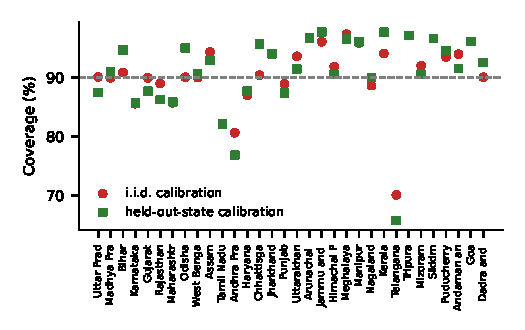
\includegraphics[width=\columnwidth]{figures/coverage_states.pdf}
\caption{Per-state coverage of YieldRank's 90\% LAC sets under leave-states-out (states with $\ge30$ test queries). The dashed line is the target.}
\label{fig:cov}
\end{figure}

\subsection{Comparison with recent methods}\label{sec:compare}

Table~\ref{tab:methods} runs \MCNMethods{} methods on the same queries, folds and calibration
sets. They are the classic baselines, \MCNPaperMethods{} reimplementations of \MCNPapers{} recent
papers \cite{dey2024,afzal2025,gunasekaran2025,ahmed2025,mahesh2026,bakr2025} with their published
hyper-parameters (unstated settings, subsampling and other deviations are listed per method in
the repository), and ranking variants of our own. The best reimplemented method,
\MCBestPaperName, reaches \MCBestPaperHitR\% on a random split but \MCBestPaperHit\% on unseen
states, against \OursHitLSO\% for YieldRank. Table~\ref{tab:ablation} shows what each component
buys on unseen states. Without the yield target (ranking by area share, i.e.\ by what farmers
already grow) Hit@1 falls to \MCAblNoYield\%. Without district history it falls to
\MCAblNoHist\%, and without the persistence term to \MCAblNoPers\%. Without the conformal step, a
single recommendation is right only \OursHitLSO\% of the time and carries no guarantee. YieldRank
trains in about \MCOursTrain\,s per fold and answers in \MCOursInfer\,ms per query.

\begin{table*}[t]
\caption{All methods on the same queries and folds (mean over 5 folds). Hit@1 for the three
splits; NDCG@3, cold-start Hit@1 and 90\% i.i.d.-LAC set coverage/size on unseen states; training
time per fold. $^{*}$/$^{**}$: differs from YieldRank, Wilcoxon $p<0.05$/$p<0.001$.}
\label{tab:methods}
\centering\scriptsize
\resizebox{\textwidth}{!}{\begin{tabular}{lccccccc}
\toprule
Method & \multicolumn{3}{c}{Hit@1 (\%)} & NDCG@3 & Cold Hit@1 & 90\% set & Train \\
\cmidrule(lr){2-4}
 & Random & States & Years & States & States & cov.\%/size & (s) \\
\midrule
CNN-LSTM (Bakr 2025)~\cite{bakr2025} & 25.7 & 20.8$^{**}$ & 24.6 & 0.755 & 18.7 & 86.8/4.49 & 20.5 \\
Crop prior & 29.0 & 20.2$^{**}$ & 27.4 & 0.743 & 18.8 & 82.8/4.25 & 0.1 \\
Persistence & 55.3 & 54.4$^{**}$ & 55.1 & 0.910 & 42.4 & 89.0/3.05 & 0.1 \\
Gaussian NB & 33.1 & 27.8$^{**}$ & 31.7 & 0.781 & 25.0 & 87.6/4.37 & 0.1 \\
Random Forest & 57.5 & 34.5$^{**}$ & 52.0 & 0.825 & 30.1 & 74.2/3.30 & 7.4 \\
XGBoost & 57.5 & 36.7$^{**}$ & 52.0 & 0.838 & 31.4 & 79.1/3.45 & 63.7 \\
MLP & 53.7 & 38.3$^{**}$ & 50.3 & 0.830 & 31.7 & 75.1/3.07 & 5.4 \\
XGBoost (Dey 2024)~\cite{dey2024} & 57.6 & 37.1$^{**}$ & 52.0 & 0.843 & 31.3 & 82.5/3.65 & 177.3 \\
Random Forest (Dey 2024)~\cite{dey2024} & 42.0 & 26.1$^{**}$ & 39.6 & 0.783 & 23.1 & 77.7/3.92 & 0.2 \\
SVM (Dey 2024)~\cite{dey2024} & 26.2 & 19.2$^{**}$ & 25.5 & 0.749 & 17.3 & 87.3/4.59 & 16.7 \\
k-NN (Dey 2024)~\cite{dey2024} & 35.5 & 24.4$^{**}$ & 32.1 & 0.763 & 21.6 & 87.9/4.47 & 0.1 \\
Decision Tree (Dey 2024)~\cite{dey2024} & 31.2 & 22.8$^{**}$ & 27.4 & 0.759 & 19.6 & 78.4/4.06 & 0.2 \\
RFXG hard vote (Afzal 2025)~\cite{afzal2025} & 45.3 & 32.7$^{**}$ & 43.4 & 0.809 & 27.9 & 87.0/4.15 & 1.3 \\
Stacking KNN+RF+NB$\to$LR (Ahmed 2025)~\cite{ahmed2025} & 48.3 & 27.4$^{**}$ & 44.0 & 0.786 & 24.7 & 75.9/3.72 & 28.5 \\
Stacking KNN+Bagging+NB$\to$LR (Ahmed 2025)~\cite{ahmed2025} & 48.0 & 28.8$^{**}$ & 43.5 & 0.789 & 25.4 & 75.6/3.68 & 23.3 \\
Hard vote LR+XGB+RF+DT+NB (Ahmed 2025)~\cite{ahmed2025} & 55.6 & 33.9$^{**}$ & 50.4 & 0.813 & 29.5 & 82.8/3.71 & 67.7 \\
CatBoost (Mahesh 2026 config)~\cite{mahesh2026} & 53.5 & 37.6$^{**}$ & 50.6 & 0.847 & 32.0 & 79.6/3.50 & 293.1 \\
LightGBM pointwise & 59.4 & 55.7$^{**}$ & 58.3 & 0.921 & 46.9 & 88.4/2.69 & 9.4 \\
LightGBM XE-NDCG ranker & 60.1 & 55.0$^{**}$ & 58.2 & 0.917 & 46.4 & 88.4/2.70 & 10.8 \\
XGBoost LambdaMART & 60.0 & 55.6$^{**}$ & 58.3 & 0.919 & 47.1 & 89.9/2.83 & 14.0 \\
LambdaMART (v4 listwise) & 59.7 & 55.4$^{**}$ & 57.9 & 0.920 & 47.1 & 89.8/2.87 & 9.5 \\
\textbf{YieldRank (ours)} & 60.0 & 56.3 & 58.8 & 0.922 & 47.4 & 87.7/2.69 & 22.8 \\
\bottomrule
\end{tabular}
}
\end{table*}

\begin{table}[t]
\caption{Ablation of YieldRank on unseen states (Hit@1 \%, NDCG@3, 90\% set coverage and size).}
\label{tab:ablation}
\centering\scriptsize
\resizebox{\columnwidth}{!}{\begin{tabular}{lcccc}
\toprule
Component removed & Hit@1 & NDCG@3 & Cover.\% & Size \\
\midrule
Full YieldRank & 56.3 & 0.922 & 87.7 & 2.69 \\
-- district history features & 27.4 & 0.788 & 69.0 & 3.13 \\
-- yield target & 23.2 & 0.772 & 89.4 & 4.60 \\
-- persistence term & 56.0 & 0.922 & 87.5 & 2.68 \\
-- listwise ranker + persistence & 55.7 & 0.921 & 88.4 & 2.69 \\
-- conformal step (top-1 only) & 56.3 & 0.922 & 56.3 & 1.00 \\
-- conformal step (fixed top-3) & 56.3 & 0.922 & 88.4 & 3.00 \\
\bottomrule
\end{tabular}
}
\end{table}

%=====================================================================
\section{Discussion and Limitations}

\textbf{What the benchmark changes.} On the near-synthetic Kaggle table, the question ``which
model is best?'' has an answer near 99\% that says little about deployment. On real district
data, three choices matter more than the classifier family. The first is the evaluation protocol:
random splits overstate the classifiers' Hit@1 by up to
\ClfDropMax{} points (YieldRank: \OursDrop) relative to unseen states. The second is the problem formulation: ranking
(query, crop) pairs by realised yield is consistently better than predicting a crop label.
A third is the feature set: climate and soil alone, the inputs of nearly every recommender in
Table~\ref{tab:lit}, barely transfer across states, and adding location-like features can
raise random-split scores while lowering out-of-state ones. A persistence rule that no prior
paper reports is a stronger baseline than any classifier, and we recommend that future work
include it.

\textbf{Limitations.} (i) Relevance is observed only for crops actually grown. We rank among
these, so the benchmark cannot score a crop a district has never tried. (ii) Yield percentile
measures comparative advantage, not profit or risk. MSP/cost-of-cultivation and groundwater
constraints \cite{sam2025,devineni2022,dangar2024} are natural re-ranking terms that we leave to
future work. (iii) Climate and soil are taken at district centroids. Season weather is the
\emph{realised} one, as in prior work, whereas a deployed system would use forecasts. Soil
is a single SoilGrids point per district (a state median for \SoilMedPct\% of rows), not a
field measurement such as a Soil Health Card. (iv) Conformal guarantees assume exchangeability of states. India's states
differ in size and history, and our per-state audit shows the guarantee is marginal, not
conditional \cite{barber2023}. (v) District boundaries changed over \YearA--\YearB, and new districts
appear as cold-start queries. (vi) All data come from one country: Indian districts, \YearA--\YearB. Whether the ranking
and calibration findings transfer to other agro-climates is untested, and no field trial has been
run.


%=====================================================================
\section{Conclusion}

Crop recommendation evaluated the way the literature does it, on an augmented table with
random splits, reports about 99\%. On \NQueries{} real Indian district-season-years and held-out
states, the same classifiers pick the best-yielding crop \BaseHitLSO\% of the time, below a
last-year persistence rule. Recasting the task as yield-grounded ranking raises this to
\OursHitLSO\% and NDCG@3 to \OursNDCGLSO. The gain is largest where history is missing.
Conformal sets calibrated on i.i.d.\ queries fall short of 90\% on unseen states. A
state-robust threshold delivers \CCSRCovLSO\% with \CCSRSizeLSO{} crops and lifts the worst state
to \SRWorstCov\%. Per-state coverage must still be audited, and the calibration set must respect
the shift. Benchmark,
code and a Colab notebook accompany the paper.


\bibliographystyle{IEEEtran}
\bibliography{../docs/research/references,extra}

\end{document}
